\documentclass[a4paper]{article}

\usepackage{a4wide}
\usepackage[utf8]{inputenc}
\usepackage[ngerman]{babel}
\usepackage{fancyhdr}
\usepackage{graphicx}
\usepackage[parfill]{parskip}
\usepackage{color}
\usepackage{url}

% fuer "deko-elemente"
\pagestyle{fancy}

% we needs moar platz
\topmargin -5mm
\headheight 20mm

% include logo in document head
\chead{
\includegraphics[width=50mm]{logo.pdf}}

% seitenzahl entfernen
\cfoot{}

% footer content
\lfoot{\small{AlphaLabs}}
\rfoot{\tiny{Alexander Drangmeister, Dennis Esders, Philipp Heisig, Robert Baruck, Stephan Wilde, Kilian Költzsch}}

% headrule
\renewcommand\headrule{
\vspace{3mm}
\footrule
}

% footrule
\renewcommand\footnoterule{\rule{\linewidth}{0pt}}

% change standard font
\usepackage[T1]{fontenc}
\newcommand{\changefont}[3]{
\fontfamily{#1} \fontseries{#2} \fontshape{#3} \selectfont}

% Tagesordnungspunkt Item
\newcommand{\TOP}[1]{\item \textbf{#1}\par}



\begin{document}
\changefont{cmss}{m}{n} %computer modern sans serif

\begin{center}
\textbf{\Large The Circle of Waste - Teilziel 3}
\end{center}

\vspace{5mm}

% ich weiss leider wirklich nicht was LaTeX hier fuer ein bescheuertes Problem hat, aber ich entschuldige mich aufrichtig fuer diesen "Format-Spam", irgendwann™ schaue ich mir das mal genauer an, so ist das ja ne zumutung m(
\definecolor{dgreen}{rgb}{0.549,0.776,0.247}
\makeatletter
\def\footrule{{
  \vskip-\footruleskip\vskip-\footrulewidth
  \color{\footrulecolor}
  \hrule\@width\headwidth\@height
  \footrulewidth\vskip\footruleskip
}}
\makeatother
\renewcommand{\footrulewidth}{3pt}
\newcommand{\footrulecolor}{dgreen}

\begin{enumerate}

\TOP{Layoutvorschlag}

\textbf{Optik}\\
Der Style lehnt an verschiedenen Müll an, so ist etwa der Hintergrund und der \glqq Spielbereich\grqq\ bräunlich bzw. gelblich an Recyclepapier angelehnt und auch alle weiteren Objekte sind so gestaltet, das sie einen unsauberen Eindruck hervorrufen.

\begin{center}
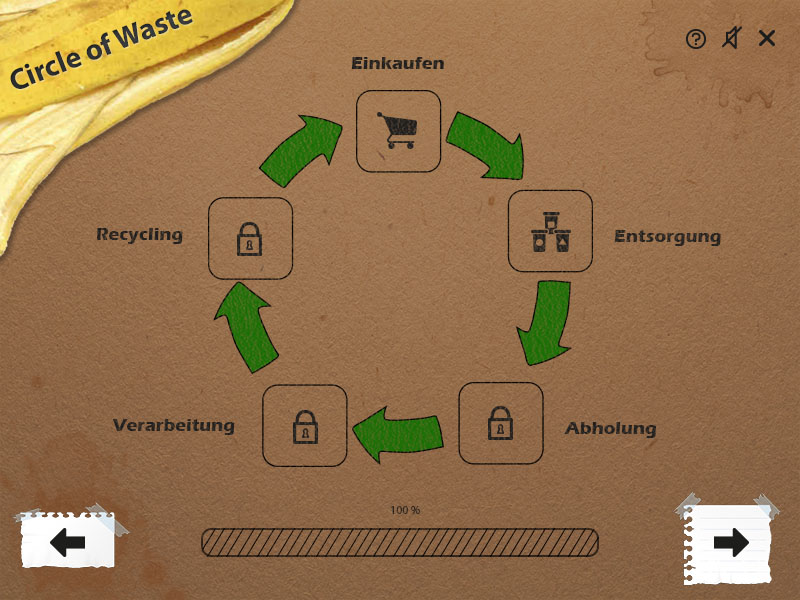
\includegraphics[width=.8\linewidth]{locks.jpg}
\end{center}

\textbf{Aufbau}\\
Unser Interface, bestehend aus dem Hintergrund, dem Namenslogo oben links, den Optionseinstellungen oben rechts, dem Fortschrittsbalken unten mittig und den Vor- und Zurückbuttons in den unteren Ecken, bleibt das ganze Spiel über bestehen. Der Bereich in der Mitte varriert.

\textbf{Menü}\\
Über die 5 Menüpunkte kann der Spieler zwischen den verschiedenen Inhalten/Leveln die er bereits freigespielt hat navigieren und außerdem anhand der Schlosssymbole erahnen, was ihm noch bevorsteht.

\textbf{Spiel}\\
Der Inhalt der einzelnen Level wird mittig, optisch von dem Hintergrund abgehoben plaziert.
Falls der Spielfluss unterbrochen wird, zB. durch den Hilfebutton, wird dies durch ausgegrauten Hintergrund dargestellt.

Einen ersten Clickdummy des Spiels kann man bereits unter \url{http://alphalbs.github.io/thecircleofwaste/game} ausprobieren.

\begin{center}
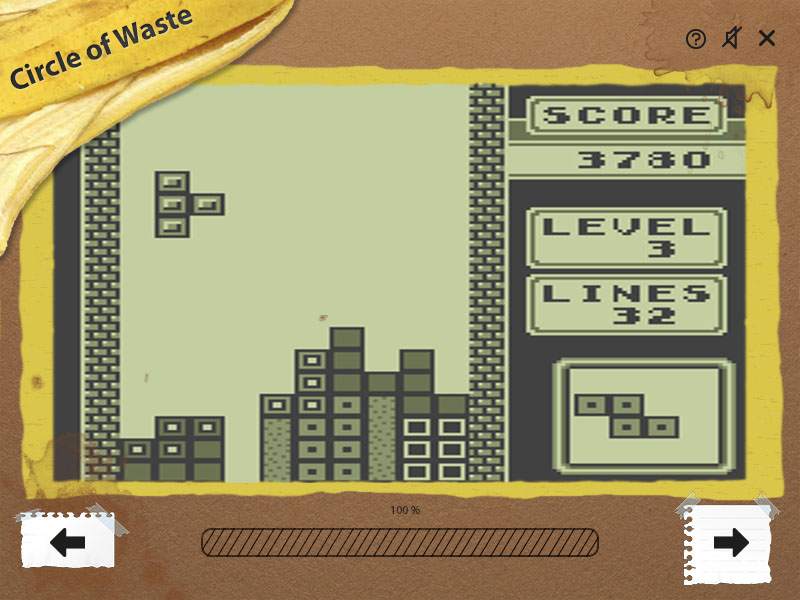
\includegraphics[width=.8\linewidth]{game.jpg}
\end{center}

Das dargestellte Spiel entspricht hier natürlich nur einem Beispiel und wird in dieser Art und Weise nicht Teil des fertigen Spiels sein.

\begin{center}
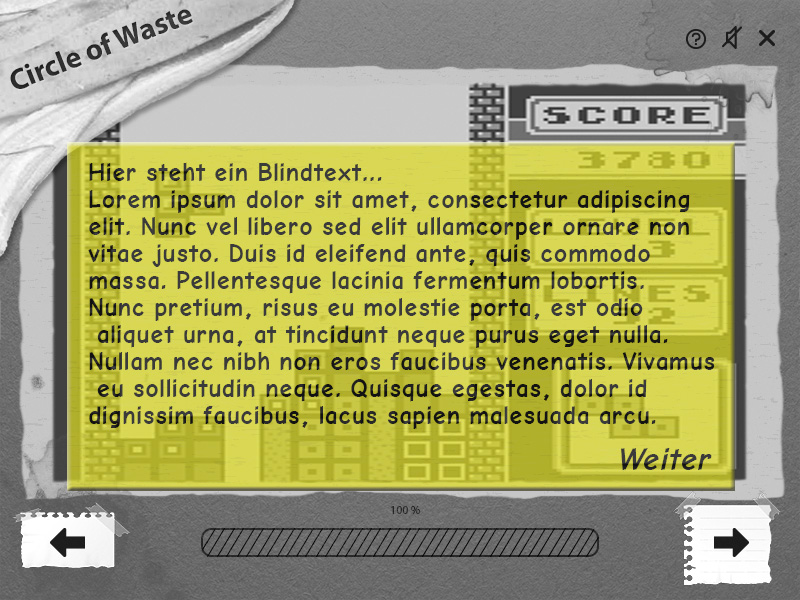
\includegraphics[width=.8\linewidth]{textoverlay.jpg}
\end{center}

\newpage

%\TOP{Detaillierte Struktur}

\TOP{Erste Inhalte}

\textbf{Verantwortungsvolles Einkaufen}
\begin{itemize}
\item Nur mit Einkaufsliste einkaufen gehen. Dies vermeidet den Kauf von unnötigen Produkten, die später verderben 
\item Verzicht auf aufwändig verpackte Produkte 
\item Bevorzugt biologisch angebaute Produkte kaufen
\item eigene Tasche oder Korb mitnehmen 
\item Mehrwegflaschen kaufen 
\end{itemize}

\textbf{Mülltrennung}\\
Wie wird Müll richtig getrennt?
\begin{itemize}
\item Restmüll
\item Altpapier
\item Leichtverpackungen
\item Altglas
\item Altkleider und Schuhe
\item Bioabfälle
\end{itemize}



\end{enumerate}


% das ist herrlich kompliziert, aber es klappt! das ist alles was zaehlt! :D
\definecolor{dgreen}{rgb}{0.549,0.776,0.247}
\makeatletter
\def\footrule{{
  \vskip-\footruleskip\vskip-\footrulewidth
  \color{\footrulecolor}
  \hrule\@width\headwidth\@height
  \footrulewidth\vskip\footruleskip
}}
\makeatother
\renewcommand{\footrulewidth}{3pt}
\newcommand{\footrulecolor}{dgreen}

\end{document}
